
To evaluate the contribution of visual information into solving the task we finetune two models in different settings: using both image and context as input and replacing image feature vector with constant input. We expect the model which has access to visual modality to perform better, which would mean that images in the composed dataset are actually relevant and useful for utterance prediction.

To train our models we utilise a prefix LM learning paradigm as opposed to usual next token prediction used to finetune BLIP on captioning tasks. We use the image and the last utterance before the image as inputs for the model and aim to predict the substituted utterance. We let the decoder use a square attention mask for the context tokens and a triangular attention mask for the utterance tokens we want to predict.

For both models we freeze the image encoder part during training for efficiency and to reduce compute cost.

Both models are trained on 4336 samples from the composed dataset, leaving 400 samples for validation, for 20 epochs with batch size of 10 samples, learning rate of 1e-5, and cosine learning rate scheduler with linear warmup (Figure \ref{fig:bleu_val}). For each setting we train 5 models initializing from different seeds for better quality estimation.

\begin{figure}[h]
    \centering
    % TODO: uncomment
    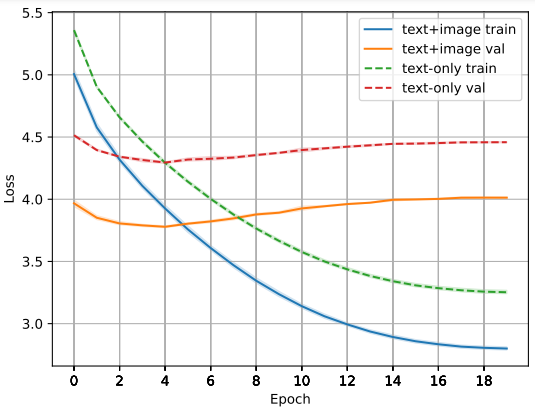
\includegraphics[width=0.49\linewidth]{sections/loss.png}
    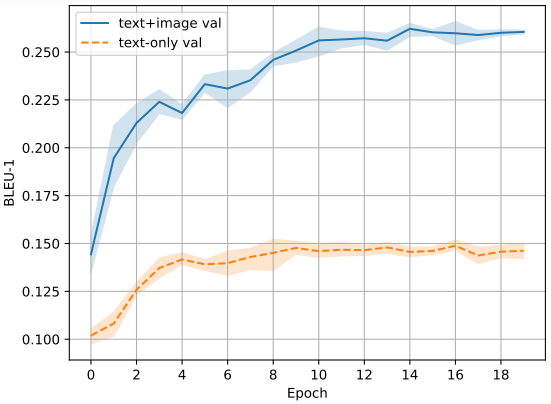
\includegraphics[width=0.49\linewidth]{sections/bleu_val.png}
    \caption{Training metrics: left figure shows train and validation loss for both finetuned BLIP models during training, right figure shows BLEU-1 metrics on validation during training.}
    \label{fig:bleu_val}
\end{figure}